\section{Facial Expression Recognition}
The development of the Pookie AI-driven robot incorporates a crucial element: detecting and interpreting user emotions, particularly stress and anxiety, using Facial Emotion Recognition (FER). This section outlines the current progress, challenges, and future approaches for designing the emotion detection system, including relevant datasets, models, and methodologies.
\subsection{Design Challenges}
Designing the input-output interaction for the robot’s FER systems presents significant challenges. Specifically:
\begin{itemize}
    \item \textbf{Defining input/output structure:} A clear operational structure needs to be established for when the robot actively listens for inputs and how it produces outputs. The temporal window during which the robot processes emotional input and when it offers feedback is still under discussion for most effective interaction.
    \item \textbf{Universality of emotions:} Stress and anxiety, being complex and abstract emotional states, are not universally exhibited across all racial or cultural groups, complicating the design of an accurate detection system, particularly for Thai users.
    \item \textbf{Dataset Challenges:} A significant hurdle in developing the FER system is the lack of available facial expression datasets for Thai people or Asians more broadly. In Thailand, researchers from Mahidol have even claimed that an open-source dataset for facial expressions in Thai ethnicity does not conventionally exist for analysts and physicians. Since accurate emotion recognition relies heavily on data representative of the target user group, this absence poses a major limitation.
\end{itemize}

Given that the most concerning challenge is related to datasets, the team is in conversation with researchers from Mahidol University to acquire a dataset from their research: \textbf{MU Face Emotion - Building a Large Dataset for Emotional Facial Expression in Psychological Domain. However, the team has not received a response}\cite{mu2022}. As a result, the team is investigating research papers to identify datasets with facial expressions most similar to those of Thai individuals. This approach would involve leveraging such datasets, followed by transfer learning techniques to fine-tune a pre-trained model on the most culturally appropriate data available. One such open source dataset is \textbf{A Chinese Face Dataset with Dynamic Expressions and Diverse Ages Synthesized by Deep Learning}\cite{han2023}, where a team of researchers created a facial expression image generation model for various Chinese faces belonging to different age groups, genders, and face structure, as shown in Figure 2.


\begin{figure}[ht]
    \centering
    \captionsetup{justification=centering}
    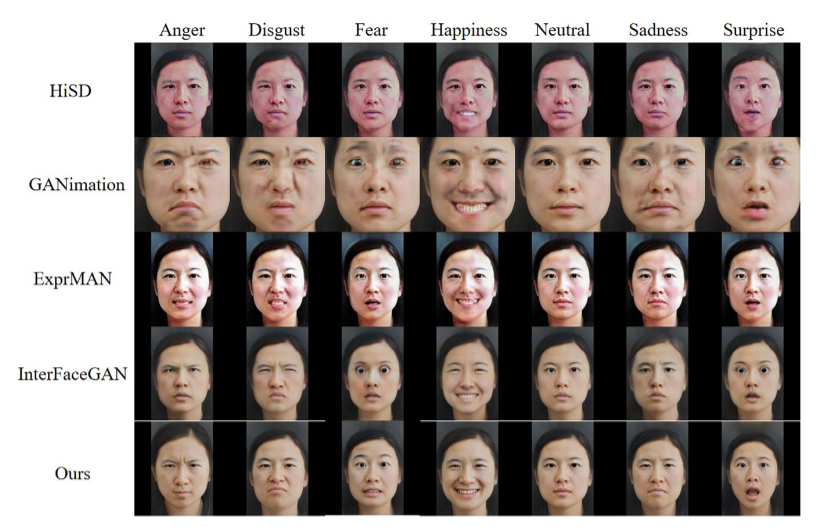
\includegraphics[width=0.75\textwidth]{faces.png}
    \caption{A Chinese Face Dataset with Dynamic Expressions and Diverse Ages Synthesized by Deep Learning (“Ours” represents the research’s proposed model)}
    \label{fig:faces}
\end{figure}
\subsection{Facial Expression Models and Stress Detection}
Facial emotion recognition is commonly based on the detection of six universal emotions: anger, disgust, fear, happiness, sadness, and surprise. These are well-researched and exhibit consistency across different cultures, making them a reliable basis for detecting emotions related to stress and anxiety. Stress and anxiety often manifest through combinations of universal emotions. For example, stress may be reflected through anger, disgust, or fear, while anxiety may be linked to fear or sadness.
Since models for detecting stress and anxiety directly are difficult to build, particularly for Asian populations, the proposed method is to detect these emotional cues by focusing on anger, disgust, and fear\cite{iceis21}. These emotions have been scientifically linked to stress, as indicated by several studies. 
\subsection{Approach for FER in Pookie}
\begin{enumerate}
    \item The FER system for Pookie will use a two-pronged approach:
    \begin{itemize}
        \item \textbf{Anxiety Detection via Speech Emotion Recognition:} Proven to be a reliable method, Pookie will detect anxiety by analyzing voice inputs, which may offer better accuracy.
        \item \textbf{Stress Detection via Facial Emotion Recognition:} Stress will be detected primarily using facial expressions linked to anger, disgust, and fear, as these are the most indicative emotions for stress according to research.
    \end{itemize}
    \item    Data Acquisition and Fine Tuning
    \begin{itemize}
        \item Select a pre-trained model (e.g., VGG19 or OpenFace) that has been trained on a universal dataset.
        \item Fine-tune the model using transfer learning by adding a new classifier layer, specifically trained on the newly acquired dataset with similar characteristics to the target population.
        \item Freeze the convolutional layers of the original model and train higher layers on the Thai dataset, ensuring it can adapt to more culturally specific facial expressions.
    \end{itemize}
    \item Program Design
    \begin{itemize}
        \item A stress classification function that monitors emotions such as anger, disgust, and fear within a defined time window.
        \item The system evaluates whether these emotions surpass a threshold, indicating stress.
    \end{itemize}

\end{enumerate}
This progress marks an important step towards enhancing Pookie's emotional intelligence and its ability to support users' mental well-being.
